\chapter{Data Preparation}
In this chapter, we introduce the data we used in this project. 

Audio event list is a list of audible events that we labelled manually.  
In this list, we mainly separate events into four big categories. 
In each category, we enumerate some common audible events we think is important and distinctive in life. 
Since we rely on audio data to train events, we download the corresponding audio clips from Sound Search Engines (SSEs). 

Scripts for movie, play, TV series are used for scene-event relation extraction. 
Because the scripts have often been labelled explicitly in some paragraphs, this information could be used for calculating their relations. 
We download scripts from various websites and combine them together to extract the scene names. 


\section{Audible Event List} 
There are already some research done on the task of building a taxonomy for audio sounds. 
An urban sound taxonomy has been built \cite{salamon2014dataset}, but it is focused only on urban environment, and the size of taxonomy is also kind of small, not having a large coverage. 
Another broad categorization of sound environments was proposed in \cite{brown2011towards}, which separate sound by broad environments. 
It has the limitation of not having specific audible events for real event detection. 
Hence, we based on the previous work, and proposed a new taxonomy for audible events. 
A new event list is then formed by extracting events from this taxonomy.  

We separate sounds basically into four groups: \textit{Human, Non-Living, Nature,} and \textit{Other Sound}. 
These four group are just a rough categorization of audible events we want to include, so the meaning of these labels are very broad to include as many specific events as possible. 

Under the \textit{Human} group, sound events are further separated into \textit{Movement}, and \textit{Non-Movement}. 
The difference of the two groups is that Movement focuses on sound made by human under some moving condition, like \textit{footstep, running, knock}. 
The intuition of this categorization is that it requires some human involvement with other items, like the ground, paper, door, etc.   
On the contrary, the \textit{Non-Movement} group contains the sound events that require less external objects or may be conducted by human themselves.

\textit{Non-Living} group was then divided into three subgroups: \textit{Equipment}, \textit{Transport}, and \textit{Material}. 
In the \textit{Equipment}, we include the basic tools we would use in office context, living environments or construction sites. 
The \textit{Transport} subgroup tries to include the transportation tools seen in modern life, which further splitted into four types: air, marine, rail and road. 
Moreover, some common materials are listed under the \textit{Material} group. 

After finishing with things highly involved with human, we turn to the natural environment to find common audible sounds. 
In this \textit{Nature} group, we further split it into animals, plants and other natural elements. 
We list common types of animals in our life and some specific birds. 
This is because the birds have a diverse location distribution, and different sounds, too. 
For example, seagulls are usually heard in sea or beach, while crows in park or forest. 
Therefore, they are distinctive for corresponding scenes, and need to be separated here. 
Usually, plants do not give out sound, so only the basic \textit{tree}, \textit{leaf} and \textit{grass} are listed here. 
The final subgroup is natural elements, which tends to appear in audio as the background sound.  


They respectively list the things in nature which may generate a sound. 

Finally, Signal and Instrument are put under Other Sound. 
They include common signals and musical instrument in life. 

\section{Audio Data}
The audio clips for the events in the eventlist we created are downloaded from SSE. 
There are many available SSEs for crawling sound clips, e.g., SoundJax\footnote{http://soundjax.com}, FindSounds\footnote{http://findsounds.com}, and Freesound\footnote{http://freesound.org}. 
We use all these SSEs to query the audio events and then download their corresponding clips. 

However, this downloading process is carried out with some filtering technique. 
Because the events we are considering suitable are ``primitive'' constituents for large audio context, their information should be covered in a comparative short time. 
So we set up a duration threshold for candidate audio clips, i.e., only downloading clips from 0.5 to 15 seconds.  

\section{Scene Context Data}
In some previous project, researchs are labelling the audible events happening in some scenes. 
This method is not only laborious, but also has a limitation for expanding to other scenes.
In this thesis, we are using a automatical way of extracting the relation between audible events and scenes.
The data we use are well-written scripts, including movies, plays, TV series, etc. 
The reason we use these scripts is because they all have a clear boundary of one ``scene''. 
In well-written scripts, whenever the plot switches to a new place, there is a sentence in the top to indicate what the current scene is. 
% script example
\begin{figure}[htb]
\centering
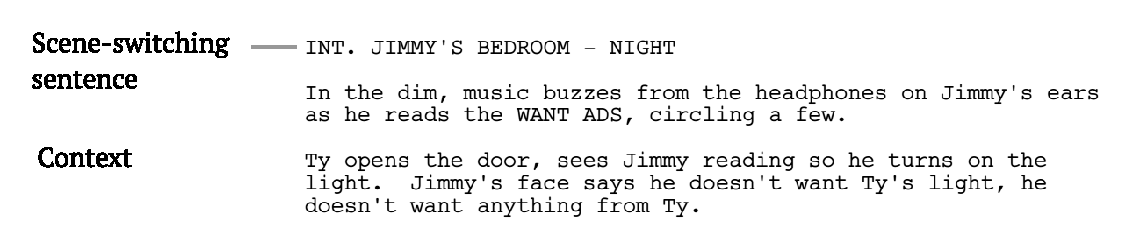
\includegraphics[scale=0.6]{figure/dataprep/script}
\caption{A Example of Script}
\label{fig:script}
\end{figure}

Figure \ref{fig:script} gives an example of what a script snippet may looks like. Usually on the top of it, there is a single sentence that specifies the location, time information for the paragraphs below it, which we would like to call as "scene-switching sentence". 
For example, in the example script, "INT. JIMMY's BEDROOM - NIGHT" is the scene-switching sentence. 
"INT" denotes this scene happens in a indoor environment. 
sometimes, "EXT" is used to denote ourdoor environment. 
In the middle of this sentence, some word phrase or sentence may be used to represent the context or scene. 
In this case, we may say this is a bedroom scene. 
Lastly, "NIGHT" or "DAY" is ued to refer the time when filmakers are shooting this script. 
When we are mining the relation between audible events and scenes, the scene-switching sentence needs to be further processed. 

Currently, there are some websites that host a collection of scripts. 
The website we used include: Simply Scripts\footnote{http://www.simplyscripts.com}, The Daily Script\footnote{http://www.dailyscript.com}, The Screenplay Database\footnote{http://www.screenplaydb.com/film/all/}, The Internet Movie Script Database(IMSDB)\footnote{http://www.imsdb.com/}, etc. 

Since the scripts are downloaded from various sites and are in different formats, we first transform the downloaded pdf or html into txt format. 
To avoid the issue of downloading the same file from different websites, the file name is checked to discard adundant scripts which have the same name with existing scripts. 
After cleaning, there are 5611 scripts in total. 

\section{Audio Scene List}
As mentioned before, well-written scripts provide a clear-defined boundary for scene switch. 
There are words words like "Cut to:", "Scene:", "INT", "EXT" to denote this kind of switching, and they are called "scene identifier".  
Following scene identifier, there usually is a short sentence or some words describing the scene the following paragraph is in. 
We call the sentence formed by scene identifier and some scene-related phrase as "scene-switching sentence"
We use the word "context" to represent the paragraphs between scene-switching sentence. \\ 

% a graph here to show a real example 

After describing the terminology we used for scripts, we need to extract the scene representing a context from the "scene-switching sentence". 
The "scene-switching sentence" sometimes contains noise, like character's name, location name, and some propositions are mixed with the actual scene name we want to extract. 
To filter out these words that could not form a scene, we use the Stanford CoreNLP \cite{manning2014corenlp}. 
Stanford CoreNLP integrates many NLP tools, including the part-of-speech (POS) tagger, the named entity recognizer (NER), the dependency parser, etc. 
It has a online demo here\footnote{http://nlp.stanford.edu:8080/corenlp/process}. 
In our case, we would use Stanford CoreNLP to eliminate the following items in the "scene-switching sentence":
\begin{itemize}
\item Time indicator (e.g. day, night, noon) 
\item Possessive terms (e.g. his, her, Jimmy's)
\item Adjectives, adverbs, determiner 
\item Location terms 
\item Non-alphabetic terms 
\end{itemize}
After these terms are filtered out, we take the words left as the scene for its following context. 
This results a file containing 104523 scenes. 
Then we merge the same scene together, and filter out those scenes with occurrence less than 50 times. 
In the end, we get a scene list of 133 scenes. 

\section{Summary}
In this section, we review our data preparation process. 
First, we build our event list by first constructing an audible event taxonomy. 
The building process of this taxonomy helps our clarify and categorize audible events. 
Then we describes how we downloaded audio data and movie, play scripts. 
Those scripts are further processed for the extraction of scenes, and we get a scene list by setting a threshold of occurrence. 
